% Provenance (never printed): old terminale S material on magmatism in
% subduction zones (volcanic arcs above the slab, water released by the slab
% and hydrous melting of the mantle wedge, andesitic volcanism and granitoid
% plutons, growth of the continental crust). Owner (Sync 0): volcanic arc,
% hydrous melting, granodiorite, batholith, continental growth. Subduction,
% slab, Wadati-Benioff zone, blueschist and eclogite are g11.06's; partial and
% decompression melting and peridotite g11.05's; andesite, diorite, rhyolite,
% pluton g11.08's; continental crust g12.01's; magma, explosive eruption Book 1's
% (g7): recalled, never redefined. Figures: figdata/grade-12/arc_magmatism.py
% (GVP volcanoes, ComCat NE Japan band, dry solidus via grade-11
% geotherm_solidus.py, wet solidus brackets of Wang 2020 and Kawamoto-Holloway 1997).
\chapter{क्षेपण क्षेत्रों पर मैग्मा-क्रिया}\label{ch:g12:subduction-magmatism}

18 मई 1980 को, सुबह 8:32 बजे, परिमाण 5.1 के एक भूकंप ने माउंट
सेंट~हेलेंस को हिला दिया। उसी क्षण ज्वालामुखी का उत्तरी पार्श्व, जो प्रतिदिन लगभग
दो मीटर बाहर की ओर फूल रहा था, खिसककर बह गया: अभिलिखित इतिहास का सबसे बड़ा मलबा-हिमस्खलन,
लगभग \qty{2.5}{km^3} चट्टान। अपने भार से मुक्त होकर, भीतर का गैस-समृद्ध मैग्मा
उस घाव से होकर बगल की ओर फट निकला, कम से कम
\qty{480}{km/h} की चाल से, और \qty{600}{km^2} में जंगलों को धराशायी कर दिया। पंद्रह
मिनट के भीतर राख का एक स्तंभ \qty{24}{km} से भी अधिक ऊँचा खड़ा था, और
उद्गार नौ घंटे चलता रहा। इकसठ लोग मारे गए या कभी नहीं मिले।
% ledger: usgs:b2-msh-1980, usgs:msh-deaths

\begin{omfigure}
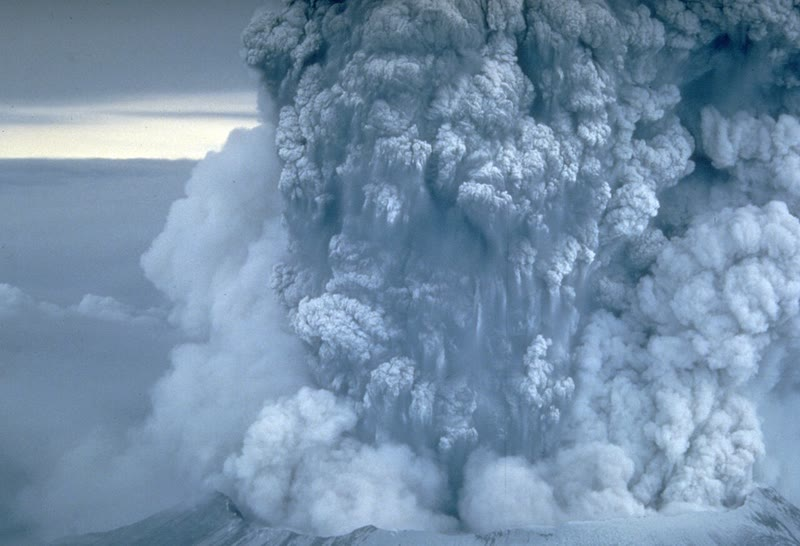
\includegraphics[width=0.55\linewidth]{images/book2/g12-swanson-st-helens-plume.jpg}

{\small 18 मई 1980 को माउंट सेंट~हेलेंस का राख-स्तंभ, जो पंद्रह मिनट से कम में
\qty{24}{km} से अधिक ऊँचा उठा। फ़ोटो डोनाल्ड
ए॰~स्वानसन, USGS (सार्वजनिक डोमेन)।}
\end{omfigure}
% ledger: photo:g12-st-helens, usgs:b2-msh-1980

माउंट सेंट~हेलेंस ज्वालामुखियों की एक पंक्ति में से एक है --- बेकर, रेनियर, हुड,
शास्ता और अन्य --- जो उस स्थान के ऊपर खड़ी है जहाँ एक छोटी महासागरीय
प्लेट, जुआन दे फ़ूका प्लेट, उत्तर अमेरिका के नीचे डूबती है। यह अध्याय
पूछता है कि ज्वालामुखी वहाँ क्यों मिलते हैं, उनके उद्गार इतनी बार हिंसक क्यों होते हैं,
और उस मैग्मा का क्या होता है जो कभी सतह तक नहीं पहुँचता।
% ledger: earle:cascades

\begin{recall}
\omterm{def:g11:subduction-zones:subduction}{क्षेपण क्षेत्र} पर \omterm{def:g11:ocean-ridges:oceanic-lithosphere}{महासागरीय स्थलमंडल} की एक प्लेट किसी दूसरी प्लेट के नीचे वापस
प्रावार में डूबती है; उसके भूकंप, \omterm{def:g11:subduction-zones:benioff}{वादाती--बेनिऑफ़ क्षेत्र},
\omterm{def:g11:subduction-zones:slab}{स्लैब} का \qty{670}{km} जितनी गहराई तक अनुसरण करते हैं
(\cref{ch:g11:subduction-zones})। प्रावार \omterm{def:g11:ocean-ridges:peridotite}{पेरिडोटाइट} से बना है; वह
ठोस है, पर ऊपर उठने वाली और कम भिंची चट्टान आंशिक रूप से पिघल सकती है,
\omterm{def:g11:ocean-ridges:partial-melting}{दाब-मुक्ति गलन} द्वारा, जैसे किसी कटक के नीचे (\cref{ch:g11:ocean-ridges})।
\omterm{def:g11:igneous-rocks:rock-names}{एंडेसाइट} बेसाल्ट और \omterm{def:g11:igneous-rocks:rock-names}{रायोलाइट} के बीच की एक \omterm{def:g11:igneous-rocks:volcanic-plutonic}{ज्वालामुखीय चट्टान} है, \omterm{def:g11:igneous-rocks:rock-names}{डायोराइट} उसकी \omterm{def:g11:igneous-rocks:volcanic-plutonic}{पातालीय}
समतुल्य, और \omterm{def:g11:igneous-rocks:intrusion}{प्लूटॉन} मैग्मा का एक बड़ा पिंड जो भूमि के नीचे ठंडा हुआ
(\cref{ch:g11:igneous-rocks})। \omterm{def:g12:continental-crust:continental-crust}{महाद्वीपीय भूपर्पटी} मोटी और हल्की है,
ऊपर ज़्यादातर ग्रेनाइटी चट्टान (\cref{ch:g12:continental-crust})। विस्फोटक
उद्गार मैग्मा को उसकी अपनी गैस से टुकड़े-टुकड़े करके उड़ा देता है (पुस्तक 1, कक्षा 7)।
\end{recall}
% ledger: tulane:magma-types, tulane:intrusions, rg14:crust

\section{ज्वालामुखीय चाप}

स्थल पर के अधिकांश सक्रिय ज्वालामुखी यादृच्छिक रूप से नहीं खड़े हैं। अंतिम हिमयुग के अंत से
उद्गार कर चुके और ग्लोबल वोल्कैनिज़्म प्रोग्राम की सूची में दर्ज 1214
ज्वालामुखियों में से 838 --- तीन में से दो से भी अधिक --- किसी \omterm{def:g11:subduction-zones:subduction}{क्षेपण क्षेत्र} के ऊपर
खड़े हैं। प्रशांत के चारों ओर वे लगभग अटूट वलय बनाते हैं, जिसे अक्सर
अग्नि-वलय कहा जाता है, और उनकी हर पंक्ति किसी खाई के समांतर,
उस प्लेट की ओर चलती है जो नहीं डूबती।
% values: n_volcanoes 1214, n_subduction 838, frac_subduction 0.690 (arc_magmatism.py)
% ledger: data:gvp, tulane:arc

\begin{omfigure}
\begin{tikzpicture}
\begin{axis}[ommap, width=\linewidth, xtick={-180,-90,...,180}, ytick={-60,0,60},
  legend style={font=\scriptsize, at={(0.5,-0.13)}, anchor=north, legend columns=3,
    /tikz/every even column/.append style={column sep=6pt}}]
\addplot[fill=omLithAlluv, draw=black!45, line width=0.2pt, forget plot] table {figdata/out/shared-geo-land.dat};
\addplot[black!70, line width=0.5pt, forget plot] table {figdata/out/shared-geo-school-subduction.dat};
\addplot[fill=black!70, draw=none, forget plot] table {figdata/out/shared-geo-school-teeth.dat};
% computed in figdata/grade-12/arc_magmatism.py; ledger: data:gvp, data:pb2002, data:ne-land
\addplot[only marks, mark=triangle*, mark size=1.1pt, black!40] table[x=lon, y=lat] {figdata/out/grade-12-arc_magmatism-world-other.dat};
\addplot[only marks, mark=triangle*, mark size=1.3pt, omThm] table[x=lon, y=lat] {figdata/out/grade-12-arc_magmatism-world-sub.dat};
\addlegendimage{black!70, line width=0.5pt}
\legend{{दूसरे ज्वालामुखी}, {क्षेपण क्षेत्र के ऊपर के ज्वालामुखी}, {खाई}}
\end{axis}
\end{tikzpicture}

{\small अंतिम हिमयुग के अंत से सक्रिय ज्वालामुखी, लाल जहाँ
वे किसी \omterm{def:g11:subduction-zones:subduction}{क्षेपण क्षेत्र} के ऊपर खड़े हैं, खाइयों के साथ (काली रेखा, त्रिभुज
ऊपर चढ़ने वाली प्लेट पर)। आँकड़े: स्मिथसोनियन ग्लोबल वोल्कैनिज़्म प्रोग्राम;
बर्ड (2003) की प्लेट-सीमाएँ; स्थल नैचुरल अर्थ से।}
\end{omfigure}
% values: n_subduction 838 of 1214 (arc_magmatism.py)

\begin{definition}[ज्वालामुखीय चाप]\label{def:g12:subduction-magmatism:arc}
\emph{ज्वालामुखीय चाप}\index{ज्वालामुखीय चाप} किसी \omterm{def:g11:subduction-zones:subduction}{क्षेपण क्षेत्र} की
ऊपर चढ़ने वाली प्लेट पर ज्वालामुखियों की एक पंक्ति है, खाई के समांतर, जो
उस स्थान के ऊपर खड़ी है जहाँ \omterm{def:g11:subduction-zones:slab}{स्लैब} लगभग सौ किलोमीटर की
गहराई तक पहुँच चुकी है। वह \emph{द्वीप-चाप} है जब वह समुद्री तली से उठता है, जैसे
जापान या इंडोनेशिया में, और महाद्वीपीय चाप जब वह किसी महाद्वीप पर खड़ा हो,
जैसे एंडीज़ या कैस्केड में।
\end{definition}
% ledger: tulane:arc, earle:arc-water, earle:cascades, sa06:slab-depth

चाप का खाई से निकटतम किनारा \textbf{ज्वालामुखीय
अग्र-रेखा} कहलाता है: उसकी खाई वाली ओर कोई भी ज्वालामुखी नहीं है। उसके नीचे
\omterm{def:g11:subduction-zones:slab}{स्लैब} कितनी गहरी है?

\begin{proposition}[ज्वालामुखीय अग्र-रेखा के नीचे की स्लैब]\label{prop:g12:subduction-magmatism:depth}
यदि \omterm{def:g11:subduction-zones:slab}{स्लैब} एक तल है जो खाई से कोण $\theta$ पर नत है, और
ज्वालामुखीय अग्र-रेखा खाई से क्षैतिज दूरी $d$ पर है, तो
अग्र-रेखा के नीचे \omterm{def:g11:subduction-zones:slab}{स्लैब} का शीर्ष इस गहराई पर है:
\[
  H = d \tan\theta .
\]
\end{proposition}

\begin{proof}
खाई के आर-पार एक ऊर्ध्वाधर काट लीजिए। \omterm{def:g11:subduction-zones:slab}{स्लैब}, सतह और
अग्र-रेखा के नीचे की ऊर्ध्वाधर रेखा एक समकोण त्रिभुज बनाते हैं, जिसका समकोण
अग्र-रेखा के नीचे है: सतह के अनुदिश की भुजा $d$ है, ऊर्ध्वाधर भुजा
$H$, और खाई पर का कोण $\theta$। इसलिए $\tan\theta = H/d$।
\end{proof}

\qty{33000}{km} लंबे चापों के अनुदिश 839 ज्वालामुखीय केंद्रों के एक संकलन ने
उनमें से हर एक के नीचे $H$ मापा: चाप के \qty{500}{km} लंबे खंडों पर औसत लेने पर
यह 72 से \qty{173}{km} तक है, माध्य \qty{105}{km}। खड़ी
\omterm{def:g11:subduction-zones:slab}{स्लैबों} के ऊपर के चाप अपनी खाई के निकट होते हैं, मंद नत \omterm{def:g11:subduction-zones:slab}{स्लैबों} के ऊपर के चाप उससे
दूर, पर उनके नीचे \omterm{def:g11:subduction-zones:slab}{स्लैब} सदा लगभग सौ किलोमीटर
नीचे होती है।
% ledger: sa06:slab-depth

\begin{method}[किसी ज्वालामुखी के नीचे स्लैब ढूँढ़ना]\label{met:g12:subduction-magmatism:slab}
\begin{enumerate}
  \item चाप के आर-पार की एक संकरी पट्टी के भूकंप लीजिए, और उनकी
        गहराई को चाप के आर-पार उनकी दूरी के सापेक्ष, वास्तविक पैमाने पर, आलेखित कीजिए।
  \item लगभग \qty{70}{km} से गहरे भूकंप रखिए: उथले भूकंप
        ऊपर चढ़ने वाली प्लेट में और दोनों प्लेटों के बीच के भ्रंश पर
        भी होते हैं।
  \item गहरे भूकंपों की रेखा खींचिए, या ज्वालामुखीय अग्र-रेखा के नीचे
        उनकी गहराई पढ़िए: वहाँ \omterm{def:g11:subduction-zones:slab}{स्लैब} की गहराई यही है।
  \item $H = d\tan\theta$ से इसकी जाँच कीजिए, $d$ को खाई से और
        नमन $\theta$ को काट पर मापकर।
\end{enumerate}
\end{method}

\begin{omfigure}
\begin{tikzpicture}
\begin{axis}[omsection, name=jp, scale only axis, width=0.8\linewidth, height=0.2857\linewidth,
  xmin=0, xmax=700, ymin=0, ymax=250, y dir=reverse,
  xlabel={\ang{138}~पू के पूर्व में दूरी (\unit{km})}, ylabel={गहराई (\unit{km})},
  xtick={0,100,...,700}, ytick={0,50,...,250}, tick label style={font=\small},
  every axis label/.append style={font=\small}]
% computed in figdata/grade-12/arc_magmatism.py; ledger: data:b2-usgs-ne-japan, data:gvp, data:pb2002
\addplot[only marks, mark=*, mark size=0.55pt, black!35] table[x=x_km, y=depth] {figdata/out/grade-12-arc_magmatism-jp-quakes.dat};
\addplot[omDef, line width=0.9pt, dashed] table[x=x_km, y=depth] {figdata/out/grade-12-arc_magmatism-jp-slab.dat};
\addplot[only marks, mark=triangle*, mark size=2.6pt, omThm] table[x=x_km, y expr=-7] {figdata/out/grade-12-arc_magmatism-jp-volc.dat};
\draw[omThm, densely dotted, line width=0.8pt] (axis cs:259.2,0) -- (axis cs:259.2,98.2);
\fill[omThm] (axis cs:259.2,98.2) circle (1.6pt);
\coordinate (front) at (axis cs:259.2,-14);
\coordinate (trench) at (axis cs:528.9,-14);
\coordinate (H) at (axis cs:262,60);
\coordinate (slab) at (axis cs:95,228);
\draw[black, line width=0.9pt] (axis cs:528.9,-12) -- (axis cs:528.9,0);
\end{axis}
\node[font=\scriptsize, anchor=south, text=omThm] at (front) {ज्वालामुखीय अग्र-रेखा (इवाते)};
\node[font=\scriptsize, anchor=south] at (trench) {जापान खाई};
\node[font=\scriptsize, anchor=west, text=omThm, fill=white, inner sep=1pt] at (H) {\qty{98}{km}};
\node[font=\scriptsize, anchor=west, text=omDef, fill=white, inner sep=1pt] at (slab) {स्लैब, लगभग \ang{20} नत};
\end{tikzpicture}

{\small उत्तर-पूर्वी जापान के आर-पार वास्तविक पैमाने पर एक काट:
\ang{37.5} और \ang{40.5}~उ के बीच परिमाण 4.5 या अधिक के भूकंप, 1976--2025 (धूसर),
उसी पट्टी के ज्वालामुखी (लाल त्रिभुज) और \qty{70}{km} से गहरे भूकंपों पर
बैठाई गई रेखा (नीली, धराशायी)। \ang{141.5}~पू के पूर्व की
उथली घटनाओं में से पाँच में से दो 2011 की हैं, मार्च के महान
भूकंप का वर्ष। आँकड़े: USGS
भूकंप-सूची; स्मिथसोनियन ग्लोबल वोल्कैनिज़्म प्रोग्राम; बर्ड (2003) की
प्लेट-सीमाएँ।}
\end{omfigure}
% values: shallow (<70 km) events east of 141.5 E: 3622, of which 1451 in 2011 (0.40); ledger usgs:tohoku
% values: jp_front_lon 141.0 (x 259.2 km), jp_trench_lon 144.12 (x 528.9), jp_front_trench_km 269.4, jp_dip_deg 19.98, jp_H_geom 98.0, bin_141_median 98.15, jp_slab_depth_front 105.6 (arc_magmatism.py)

\begin{example}[उत्तर-पूर्वी जापान]\label{ex:g12:subduction-magmatism:japan}
चित्र की पट्टी में सबसे पूर्वी ज्वालामुखी इवाते है, \ang{141.0}~पू पर,
और जापान खाई \ang{144.1}~पू पर है। वहाँ देशांतर का एक अंश
$111.2\cos\ang{39} \approx \qty{86.4}{km}$ है, इसलिए $d \approx 3.12 \times 86.4
\approx \qty{270}{km}$। गहरे भूकंप लगभग \ang{20} नत हैं, और
\[
  H = 270 \times \tan\ang{20} \approx \qty{98}{km}.
\]
अग्र-रेखा के ठीक नीचे पड़े \qty{70}{km} से गहरे भूकंपों की
माध्यिका गहराई \qty{98}{km} है: दोनों सहमत हैं, संसार के
औसत के निकट।
\end{example}
% values: km_per_deg_lon 86.415, jp_front_trench_km 269.4, jp_dip_deg 19.98, jp_H_geom 97.98, bin_141_median 98.15 (arc_magmatism.py)

\section{जल प्रावार को पिघलाता है}

किसी चाप के नीचे \omterm{def:g11:subduction-zones:slab}{स्लैब} ठंडी है, और उसके ऊपर की \omterm{def:g11:ocean-ridges:oceanic-lithosphere}{महासागरीय भूपर्पटी} भी:
वह पिघल नहीं सकती। मैग्मा को \omterm{def:g11:subduction-zones:slab}{स्लैब} के ऊपर के गरम प्रावार,
\textbf{प्रावार-कील}, से आना चाहिए। पर कील ऊपर नहीं उठ रही, इसलिए वह
दाब-मुक्ति से नहीं पिघल सकती, जैसे वह किसी कटक के नीचे पिघलती है। कोई और चीज़ उसका गलन-
तापमान घटाती है: जल।
% ledger: earle:settings (subducted crust stays cool), earle:flux-melting, earle:arc-water

\omterm{def:g11:ocean-ridges:oceanic-lithosphere}{महासागरीय भूपर्पटी} जिस कटक पर बनती है, उसके निकट समुद्री जल से तर हो जाती है, और
उस जल का बहुत-सा भाग उसके खनिजों के भीतर बंद हो जाता है, सबसे अधिक
सर्पेंटाइन में, जो भूपर्पटी के ओलिवीन और पाइरॉक्सीन से बनता है। जैसे-जैसे \omterm{def:g11:subduction-zones:slab}{स्लैब}
डूबती और गरम होती है, ये खनिज टूटते हैं और अपना जल छोड़ देते हैं।
जल ऊपर की कील के गरम \omterm{def:g11:ocean-ridges:peridotite}{पेरिडोटाइट} में उठता है।
% ledger: earle:arc-water, tulane:arc

\begin{definition}[जलीय गलन]\label{def:g12:subduction-magmatism:hydrous-melting}
\emph{जलीय गलन}\index{जलीय गलन} (या गालक-प्रेरित गलन) किसी चट्टान का
जल जुड़ने से होने वाला \omterm{def:g11:ocean-ridges:partial-melting}{आंशिक गलन} है, जो उस
तापमान को घटा देता है जिस पर चट्टान पिघलना शुरू करती है।
\end{definition}
% ledger: earle:flux-melting, earle:arc-water

किसी दिए गए दाब पर वह तापमान जिस पर कोई चट्टान पिघलना शुरू करती है, उसका
\textbf{ठोसांक} है। शुष्क \omterm{def:g11:ocean-ridges:peridotite}{पेरिडोटाइट} के लिए यह भली-भाँति ज्ञात है; जल के साथ इसे
मापना कहीं कठिन है, और प्रकाशित मान अब भी 200 से
\qty{600}{\celsius} तक भिन्न हैं। सबसे नए प्रयोग इसे \qty{3}{GPa} पर,
लगभग \qty{95}{km} नीचे, 950 और \qty{1000}{\celsius} के बीच रखते हैं, और 5 से \qty{11}{GPa} तक
\qty{1000}{\celsius} से ठीक ऊपर। \qty{3}{GPa} पर शुष्क \omterm{def:g11:ocean-ridges:peridotite}{पेरिडोटाइट}
केवल लगभग \qty{1470}{\celsius} पर पिघलना शुरू करता है: जल ठोसांक को
लगभग \qty{500}{\celsius} घटा देता है।
% values: dry_T_3gpa 1473.4, dry_minus_wet_3gpa 498, z_3gpa_km 95.2, dry_minus_wet_5gpa 658 (arc_magmatism.py)
% ledger: hirschmann:solidus, wang20:wet-solidus, kh97:wet-solidus, data:prem, earth:gmean

\begin{omfigure}
\begin{tikzpicture}
\begin{axis}[omrecord, name=sol, scale only axis, width=0.62\linewidth, height=6.2cm,
  xmin=700, xmax=1900, ymin=0, ymax=230, y dir=reverse,
  xlabel={तापमान (\unit{\celsius})}, ylabel={गहराई (\unit{km})},
  xtick={800,1000,...,1800}, ytick={0,50,...,200}, axis y line*=left]
% computed in figdata/grade-12/arc_magmatism.py (dry: Hirschmann 2000 with PREM pressures; wet: Wang 2020, Kawamoto-Holloway 1997)
\addplot[omProp, line width=1.2pt] table[x=T_dry, y=depth_km] {figdata/out/grade-12-arc_magmatism-solidus.dat};
\addplot[omDef, line width=2.4pt] coordinates {(950,95.24) (1000,95.24)};
\addplot[omDef, line width=1.2pt] coordinates {(1000,155.6) (1000,216.3)};
\draw[-{Stealth}, black!70, line width=0.8pt] (axis cs:1460,95.24) -- (axis cs:1015,95.24);
\coordinate (gap) at (axis cs:1240,95.24);
\coordinate (dry) at (axis cs:1600,40);
\coordinate (wet) at (axis cs:1015,190);
\coordinate (wet3) at (axis cs:975,90);
\end{axis}
\begin{axis}[scale only axis, width=0.62\linewidth, height=6.2cm, at={(sol.south west)}, anchor=south west,
  xmin=700, xmax=1900, ymin=0, ymax=230, y dir=reverse, axis x line=none, axis y line*=right,
  axis line style={-}, ylabel={दाब (\unit{GPa})},
  ytick={34.9,65.1,95.2,125.5,155.6,185.9,216.3}, yticklabels={1,2,3,4,5,6,7},
  every axis label/.append style={font=\small}, tick label style={font=\small}]
% pressure ticks at the PREM depths of 1-7 GPa (arc_magmatism.depth_at_pressure)
\end{axis}
\node[font=\scriptsize, anchor=south] at ([yshift=2pt]gap) {लगभग \qty{500}{\celsius}};
\node[font=\scriptsize, text=omProp, anchor=west, align=left] at (dry) {शुष्क पेरिडोटाइट\\पिघलना शुरू करता है};
\node[font=\scriptsize, text=omDef, anchor=west, align=left] at (wet) {जल के साथ: \qty{1000}{\celsius}\\से ठीक ऊपर};
\node[font=\scriptsize, text=omDef, anchor=south] at ([yshift=2pt]wet3) {950--1000};
\end{tikzpicture}

{\small वह तापमान जिस पर प्रावार का \omterm{def:g11:ocean-ridges:peridotite}{पेरिडोटाइट} पिघलना शुरू करता है, गहराई के
सापेक्ष: शुष्क (नारंगी) और जल से संतृप्त (नीला, अब तक मापे गए दो
परास)। चापों के नीचे \omterm{def:g11:subduction-zones:slab}{स्लैब} की गहराई पर, लगभग \qty{100}{km}, जल
इसे लगभग \qty{500}{\celsius} घटा देता है। स्रोत: हिर्शमान (2000),
PREM घनत्वों के साथ; वांग और अन्य (2020); कावामोटो और हॉलोवे (1997)।}
\end{omfigure}
% values: dry_T_3gpa 1473.4, dry_T_100km 1489.4, P_100km_gpa 3.157 (arc_magmatism.py)

इस तरह जल वह करता है जो अकेले गरम करना नहीं कर सकता था: वह गरम
कील के एक भाग को पिघला देता है। मैग्मा, अपने चारों ओर के ठोस प्रावार से हल्का, सतह की ओर
उठता है; कुछ उद्गार में निकलता है, कहीं अधिक भूमि के नीचे रहकर ठंडा होता है।
वह स्थान जहाँ जल मुक्त होता है, और जहाँ उसके ऊपर की कील भीगने पर पिघलने लायक
गरम है, वही ज्वालामुखीय अग्र-रेखा को \omterm{def:g11:subduction-zones:slab}{स्लैब} से लगभग सौ किलोमीटर
ऊपर तय करता है।
% ledger: earle:arc-water, tulane:arc, sa06:slab-depth, wang20:wet-solidus (position of the volcanic front controlled by melting in the wedge)

\begin{omfigure}
\begin{tikzpicture}[x=1cm, y=1cm, font=\scriptsize]
  % mantle
  \fill[omLithPeridotite!45] (0,-0.9) -- (7.4,-0.9) -- (7.5,-0.85) -- (6.5,-1.6) -- (5.5,-2.6) -- (4.5,-3.8)
    -- (4.25,-4.3) -- (0,-4.3) -- cycle;
  % sea and overriding continental crust
  \fill[omSea] (8.0,0) -- (12,0) -- (12,-0.4) -- (8.5,-0.4) -- cycle;
  \fill[omLithGranite!55] (0,0.1) -- (8.0,0.1) -- (8.5,-0.4) -- (7.5,-0.85) -- (7.4,-0.9) -- (0,-0.9) -- cycle;
  % the slab
  \fill[omLithBasalt!45, draw=black!60] (12,-0.4) -- (8.5,-0.4) -- (7.5,-0.85) -- (6.5,-1.6) -- (5.5,-2.6) -- (4.5,-3.8)
    -- (4.25,-4.3) -- (5.15,-4.3) -- (5.2,-4.3) -- (6.15,-3.15) -- (7.1,-2.2) -- (8.0,-1.55) -- (8.9,-1.2) -- (12,-1.2) -- cycle;
  \node at (10.4,-0.8) {महासागरीय स्थलमंडल};
  \node[anchor=west] at (6.0,-3.4) {डूबती स्लैब};
  % melting in the wedge, rising magma, plutons, volcano
  \fill[omThm!35, draw=omThm, densely dashed] (5.2,-1.75) ellipse (0.6 and 0.3);
  \node[omThm] at (5.2,-1.75) {गलन};
  \foreach \y in {-1.3,-1.05} \fill[omThm!80] (5.2,\y) circle (0.07);
  \fill[omLithGranite, draw=black!60] (4.75,-0.55) ellipse (0.42 and 0.2);
  \fill[omLithGranite, draw=black!60] (5.65,-0.4) ellipse (0.32 and 0.16);
  \node[anchor=east] at (4.25,-0.55) {प्लूटॉन};
  \draw[omThm, line width=1pt] (5.2,0.1) -- (5.2,-0.85);
  \fill[black!65] (4.75,0.1) -- (5.2,0.75) -- (5.65,0.1) -- cycle;
  \node[anchor=south] at (5.2,0.8) {ज्वालामुखी};
  % water released by the slab
  \foreach \x/\y in {6.5/-1.6, 6.0/-2.1, 5.6/-2.5}
    \draw[omDef, -{Stealth}, line width=0.7pt, decorate, decoration={snake, amplitude=0.6pt, segment length=4pt, post length=1.5mm}]
      (\x,\y) -- ++(-0.3,0.3);
  \draw[omDef, line width=0.3pt] (7.5,-2.75) -- (6.35,-2.0);
  \node[omDef, anchor=west, align=left] at (7.5,-2.75) {स्लैब द्वारा\\छोड़ा गया जल};
  % labels and depth scale
  \node at (1.8,-0.4) {महाद्वीपीय भूपर्पटी};
  \node[black!70, align=center] at (2.3,-3.6) {गरम प्रावार-कील\\(पेरिडोटाइट)};
  \node[anchor=south] at (8.5,0.12) {खाई};
  \draw[black!60, |-|] (0.4,0.1) -- node[left, align=right] {लगभग\\\qty{100}{km}} (0.4,-2.96);
  \draw[black!45, densely dotted] (0.4,-2.96) -- (5.2,-2.96);
  \fill[black!70] (5.2,-2.96) circle (1.3pt);
  \draw[black!45, densely dotted] (5.2,-2.96) -- (5.2,-2.05);
\end{tikzpicture}

{\small \omterm{def:g11:subduction-zones:subduction}{क्षेपण क्षेत्र} पर मैग्मा-क्रिया (योजनाबद्ध, पैमाने पर नहीं)। जैसे-जैसे \omterm{def:g11:subduction-zones:slab}{स्लैब}
गरम होती है, उसके खनिज अपना जल छोड़ते हैं, जो गरम प्रावार-कील में
उठता है और उसे आंशिक रूप से पिघला देता है। मैग्मा ऊपर उठता है: उसका कुछ भाग
ज्वालामुखियों से निकलता है, अधिक भाग भूपर्पटी में \omterm{def:g11:igneous-rocks:intrusion}{प्लूटॉनों} के रूप में ठंडा होता है।}
\end{omfigure}
% ledger: earle:arc-water, earle:flux-melting, tulane:arc, tulane:ridge-rocks, sa06:slab-depth

\section{एंडेसाइट और ग्रैनोडायोराइट}

भीगे \omterm{def:g11:ocean-ridges:peridotite}{पेरिडोटाइट} के पहले गलित बेसाल्टी नहीं होते।
\qty{1}{GPa} पर प्रयोगों में जल-संतृप्त \omterm{def:g11:ocean-ridges:peridotite}{पेरिडोटाइट} एंडेसाइटी
संघटन के गलित देता है। चाप की मोटी भूपर्पटी से होकर ऊपर उठते हुए मैग्मा ठंडे होने के साथ
बदलते भी हैं, बेसाल्टी से एंडेसाइटी और रायोलाइटी की ओर। इसलिए चाप-मैग्मा
कटकों के बेसाल्टों की अपेक्षा सिलिका में अधिक समृद्ध होते हैं --- एंडेसाइटी मैग्मा
में वह 55 से \qty{65}{\percent} होती है --- और वे उस जल को ढोते हैं जिसने उन्हें
बनाया।
% ledger: kh97:wet-solidus (andesitic melts at 1 GPa), tulane:eruptions, tulane:ridge-rocks, tulane:magma-types

ये दोनों गुण उनके उद्गारों को हिंसक बनाते हैं। मैग्मा में जितनी अधिक सिलिका,
वह उतना ही अधिक श्यान होता है, और उसकी गैस का निकलना उतना ही कठिन; विस्फोटक
उद्गारों को ऊँची गैस-मात्रा और ऊँची श्यानता से बढ़ावा मिलता है, जैसे
एंडेसाइटी और रायोलाइटी मैग्मा में। लगभग सभी स्तरित ज्वालामुखी
\omterm{def:g11:subduction-zones:subduction}{क्षेपण क्षेत्रों} के ऊपर खड़े हैं: हज़ारों मीटर ऊँचे और \qty{20}{km} तक
चौड़े शंकु, 10 से 30 अंश की ढलानों वाले, जिनके उद्गार शांत
लावा-प्रवाहों से लेकर विस्फोटों तक होते हैं। माउंट सेंट~हेलेंस के नीचे लगभग \qty{1}{km} चौड़ा एक मैग्मा कक्ष
लगभग 6 से \qty{14}{km} की गहराई तक फैला है।
% ledger: tulane:magma-types, tulane:eruptions, earle:composite

अधिकांश चाप-मैग्मा कभी उद्गार में नहीं निकलता। वह भूपर्पटी में धीरे-धीरे ठंडा होकर
स्थूलकणी चट्टानों में क्रिस्टलित होता है।

\begin{definition}[ग्रैनोडायोराइट]\label{def:g12:subduction-magmatism:granodiorite}
\emph{ग्रैनोडायोराइट}\index{ग्रैनोडायोराइट} ग्रेनाइट जैसी एक स्थूलकणी \omterm{def:g11:igneous-rocks:volcanic-plutonic}{पातालीय चट्टान} है,
पर पोटैशियम फ़ेल्डस्पार की अपेक्षा अधिक प्लेजियोक्लेज़ के साथ: उसके हल्के खनिजों का 20 से
\qty{60}{\percent} क्वार्ट्ज़ है, और उसके फ़ेल्डस्पार का 65 से
\qty{90}{\percent} प्लेजियोक्लेज़; उसमें अक्सर बायोटाइट
या हॉर्नब्लेंड होता है।
\end{definition}
% ledger: bgs:granodiorite

\begin{omfigure}
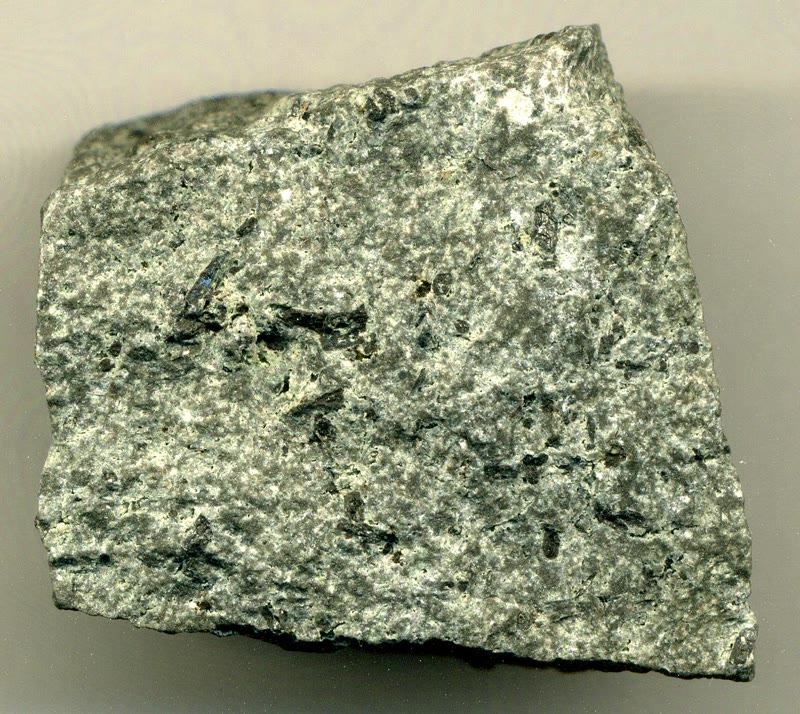
\includegraphics[height=4.4cm]{images/book2/g12-stjohn-andesite.jpg}\hspace{0.03\linewidth}%
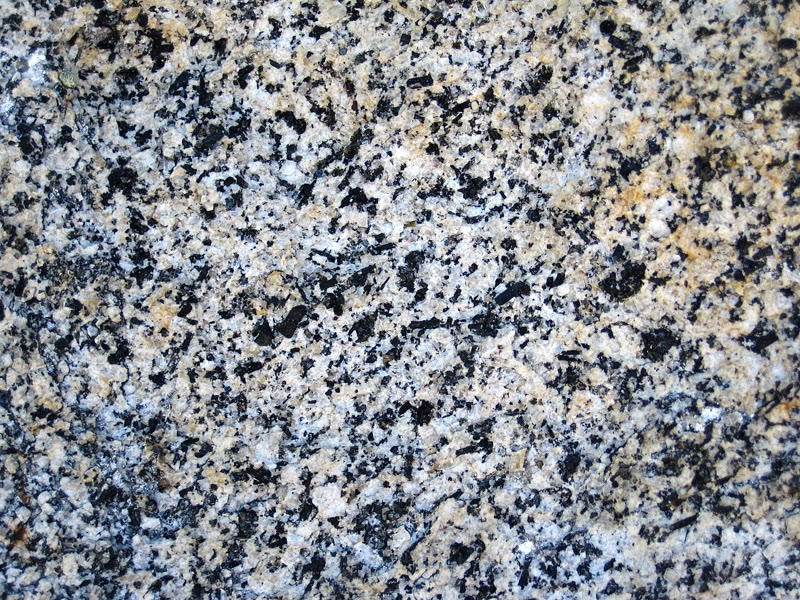
\includegraphics[height=4.4cm]{images/book2/g12-stjohn-granodiorite.jpg}

{\small बाएँ: \omterm{def:g11:igneous-rocks:rock-names}{एंडेसाइट}, चापों की एक सूक्ष्मकणी \omterm{def:g11:igneous-rocks:volcanic-plutonic}{ज्वालामुखीय चट्टान}। दाएँ:
सिएरा नेवादा का \omterm{def:g12:subduction-magmatism:granodiorite}{ग्रैनोडायोराइट}, सफ़ेद प्लेजियोक्लेज़, धूसर क्वार्ट्ज़ और
काले बायोटाइट और हॉर्नब्लेंड के साथ। फ़ोटो जेम्स सेंट~जॉन (CC~BY~2.0)।}
\end{omfigure}
% ledger: photo:g12-andesite, photo:g12-granodiorite

औसतन ऊपरी \omterm{def:g12:continental-crust:continental-crust}{महाद्वीपीय भूपर्पटी} में लगभग \qty{67}{\percent}
\ce{SiO2} होता है: वह \omterm{def:g11:igneous-rocks:felsic-mafic}{फ़ेल्सिक} है, उन ग्रेनाइटों की तरह जिन्हें चाप अपने
\omterm{def:g12:subduction-magmatism:batholith}{बैथोलिथों} में भारी मात्रा में बनाते हैं।
% ledger: rg14:crust (upper crust SiO2 66.6 wt %), tulane:magma-types, tulane:intrusions

\begin{definition}[बैथोलिथ]\label{def:g12:subduction-magmatism:batholith}
\emph{बैथोलिथ}\index{बैथोलिथ} \omterm{def:g11:igneous-rocks:volcanic-plutonic}{पातालीय चट्टान} का एक बड़ा पिंड है जो, जहाँ अपरदन ने उसे
अनावृत किया है, \qty{100}{km^2} से अधिक क्षेत्र ढकता है। वह वहाँ बनता है जहाँ बहुत-से
\omterm{def:g11:igneous-rocks:intrusion}{प्लूटॉन}, एक के बाद एक अंतर्वेधित होकर, सतह के नीचे जुड़ जाते हैं।
\end{definition}
% ledger: earle:batholith, tulane:intrusions

संसार के सबसे बड़े \omterm{def:g12:subduction-magmatism:batholith}{बैथोलिथों} में से एक, तटीय प्लूटॉनी संकुल, प्रशांत तट के अनुदिश
पश्चिमी कनाडा के वैंकूवर क्षेत्र से
दक्षिण-पूर्वी अलास्का तक फैला है। कैलिफ़ोर्निया का सिएरा नेवादा \omterm{def:g12:subduction-magmatism:batholith}{बैथोलिथ} एक
\omterm{def:g11:subduction-zones:subduction}{क्षेपण क्षेत्र} के ऊपर बना; योसेमिटी में उसके अधिकांश ग्रेनाइट
क्रिटेशस में, 105 से 85 मिलियन वर्ष पहले, क्रिस्टलित हुए। उनके ऊपर की चट्टानें
कई मिलियन वर्षों में घिसकर हट गईं, और जो \omterm{def:g11:igneous-rocks:intrusion}{प्लूटॉन} गहरे में ठंडे हुए थे, वे अब
पर्वत बनाते हैं।
% ledger: earle:batholith, nps:yosemite, photo:g12-sierra-nevada (St. John description), ics:base.Cretaceous

\begin{omfigure}
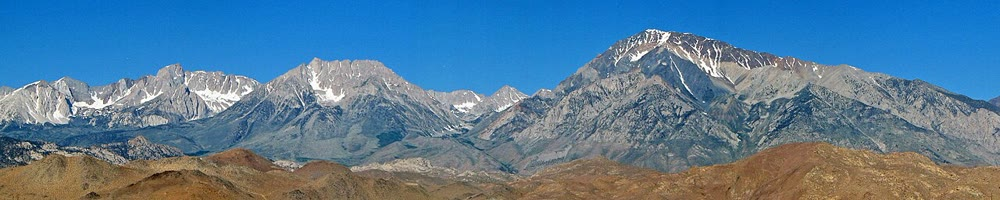
\includegraphics[width=0.94\linewidth]{images/book2/g12-stjohn-sierra-nevada-batholith.jpg}

{\small पूर्व से दिखता सिएरा नेवादा: सिएरा नेवादा \omterm{def:g12:subduction-magmatism:batholith}{बैथोलिथ} का ग्रेनाइट और
\omterm{def:g12:subduction-magmatism:granodiorite}{ग्रैनोडायोराइट}, जो क्रिटेशस में एक \omterm{def:g11:subduction-zones:subduction}{क्षेपण क्षेत्र} के ऊपर गहरे में
क्रिस्टलित हुआ। फ़ोटो जेम्स सेंट~जॉन
(CC~BY~2.0)।}
\end{omfigure}
% ledger: photo:g12-sierra-nevada, nps:yosemite

\section{महाद्वीप कैसे बढ़ते हैं}

\begin{definition}[महाद्वीपीय वृद्धि]\label{def:g12:subduction-magmatism:continental-growth}
\emph{महाद्वीपीय वृद्धि}\index{महाद्वीपीय वृद्धि} प्रावार से बनी नई
\omterm{def:g12:continental-crust:continental-crust}{महाद्वीपीय भूपर्पटी} का जुड़ना है, ज़्यादातर चापों की मैग्मा-क्रिया द्वारा।
महाद्वीपों की शुद्ध वृद्धि वह जोड़ है, उसमें से वह \omterm{def:g12:continental-crust:continental-crust}{महाद्वीपीय भूपर्पटी} घटाकर
जो प्रावार में लौट जाती है।
\end{definition}
% ledger: sv09:growth, ss09:balance

महाद्वीपों की हल्की चट्टान चापों पर ही बनती है। चाप आज जितना
मैग्मा जोड़ते हैं, उसके अनुमान द्वीप-चापों पर प्रति वर्ष लगभग \qty{1.5}{km^3}
और महाद्वीपीय चापों पर प्रति वर्ष \qty{1.0}{km^3} हैं; दीर्घ काल पर औसत लेने पर,
प्रति वर्ष लगभग \qty{2.7}{km^3}। पर \omterm{def:g11:subduction-zones:subduction}{क्षेपण क्षेत्र} \omterm{def:g12:continental-crust:continental-crust}{महाद्वीपीय
भूपर्पटी} को वापस प्रावार में भी ले जाते हैं: \omterm{def:g11:subduction-zones:slab}{स्लैब} के साथ नीचे ले जाया गया अवसाद और
ऊपर चढ़ने वाली प्लेट के नीचे से खुरचे गए टुकड़े, प्रति वर्ष लगभग \qty{3.2}{km^3}।
दोनों निकट हैं, और पिछले कई सौ मिलियन वर्षों में महाद्वीपों की शुद्ध वृद्धि
शून्य, या ऋणात्मक भी, रही हो सकती है।
% ledger: sv09:growth, ss09:balance

महाद्वीप अपने किनारों पर एक और ढंग से भी बढ़ते हैं। \omterm{def:g12:continental-crust:continental-crust}{महाद्वीपीय भूपर्पटी} इतनी
हल्की है कि उसका \omterm{def:g11:subduction-zones:subduction}{क्षेपण} नहीं हो सकता, इसलिए जब कोई प्लेट किसी महाद्वीप को खाई में ले आती है, तो
दोनों महाद्वीप एक टक्कर में आपस में जुड़ जाते हैं
(\cref{ch:g12:mountain-building})। हर महाद्वीप का एक पुराना क्रोड, एक \omterm{def:g12:continental-crust:craton}{क्रेटन}, होता है,
जो नई चट्टानों की पट्टियों से घिरा होता है, पूर्व पर्वत-पट्टियों के विकृत
\omterm{def:g12:continental-crust:root}{मूल}, जो एक के बाद एक उसके किनारों पर जुड़ी हैं
(\cref{ch:g12:continental-crust})।
% ledger: tulane:no-subduct (continental crust too buoyant to subduct), earle:collision, tulane:cratons

\section{अभ्यास}

\begin{exercise}[$\star$]\label{exo:g12:subduction-magmatism:1}
शब्द बताइए: (a) किसी खाई के समांतर ज्वालामुखियों की एक पंक्ति, उस प्लेट पर
जो नहीं डूबती; (b) किसी चट्टान में जल जोड़ने से होने वाला गलन; (c) पोटैशियम
फ़ेल्डस्पार से अधिक प्लेजियोक्लेज़ और \qty{20}{\percent} से अधिक क्वार्ट्ज़ वाली एक
\omterm{def:g11:igneous-rocks:volcanic-plutonic}{पातालीय चट्टान}; (d) \qty{100}{km^2} से बड़ा \omterm{def:g11:igneous-rocks:volcanic-plutonic}{पातालीय चट्टान} का
एक पिंड; (e) प्रावार से बनी नई \omterm{def:g12:continental-crust:continental-crust}{महाद्वीपीय भूपर्पटी} का
जुड़ना।
\end{exercise}

\begin{exercise}[$\star$]\label{exo:g12:subduction-magmatism:2}
18 मई 1980 को माउंट सेंट~हेलेंस का राख-स्तंभ 15 मिनट से कम में \qty{24}{km} से
अधिक ऊँचा उठा। (1) उसकी न्यूनतम माध्य उठान-चाल,
\unit{km/h} और \unit{m/s} में, क्या थी? (2) इसकी तुलना पार्श्व
विस्फोट की चाल, कम से कम \qty{480}{km/h}, से कीजिए।
\end{exercise}

\begin{exercise}[$\star$]\label{exo:g12:subduction-magmatism:3}
अंतिम हिमयुग के अंत से सक्रिय, सूची के 1214 ज्वालामुखियों में से
838 किसी \omterm{def:g11:subduction-zones:subduction}{क्षेपण क्षेत्र} के ऊपर खड़े हैं। (1) यह कितना प्रतिशत है? (2) ये ज्वालामुखी
खाई की किस ओर हैं? (3) खाई और ज्वालामुखीय अग्र-रेखा के बीच कोई ज्वालामुखी
क्यों नहीं है?
\end{exercise}

\begin{exercise}[$\star$]\label{exo:g12:subduction-magmatism:4}
एक स्थूलकणी चट्टान में \qty{25}{\percent} क्वार्ट्ज़, \qty{45}{\percent}
प्लेजियोक्लेज़, \qty{15}{\percent} पोटैशियम फ़ेल्डस्पार और \qty{15}{\percent}
बायोटाइट और हॉर्नब्लेंड है। (1) उसके फ़ेल्डस्पार का कितना अंश प्लेजियोक्लेज़ है?
(2) क्या यह \omterm{def:g12:subduction-magmatism:granodiorite}{ग्रैनोडायोराइट} है?
\end{exercise}

\begin{exercise}[$\star$]\label{exo:g12:subduction-magmatism:5}
दो कारण बताइए कि चापों के ज्वालामुखी कटकों के ज्वालामुखियों की अपेक्षा अधिक विस्फोटक ढंग से
क्यों उद्गार करते हैं।
\end{exercise}

\begin{exercise}[$\star\star$]\label{exo:g12:subduction-magmatism:6}
(1) एक ज्वालामुखीय अग्र-रेखा अपनी खाई से \qty{150}{km} दूर है, एक ऐसी \omterm{def:g11:subduction-zones:slab}{स्लैब} के ऊपर जो
\ang{35} नत है। उसके नीचे \omterm{def:g11:subduction-zones:slab}{स्लैब} कितनी गहरी है? (2) इसकी तुलना
\qty{105}{km} के औसत से कीजिए।
\end{exercise}

\begin{exercise}[$\star\star$]\label{exo:g12:subduction-magmatism:7}
मान लीजिए हर ज्वालामुखीय अग्र-रेखा के नीचे \omterm{def:g11:subduction-zones:slab}{स्लैब} \qty{105}{km} पर है। जब \omterm{def:g11:subduction-zones:slab}{स्लैब} \ang{20} नत हो,
और जब वह \ang{45} नत हो, तो अग्र-रेखा खाई से कितनी दूर होती है?
इससे आपको क्या पता चलता है कि चाप को कहाँ खोजना चाहिए?
\end{exercise}

\begin{exercise}[$\star\star$]\label{exo:g12:subduction-magmatism:8}
\qty{100}{km} पर दाब लगभग \qty{3.16}{GPa} है। (1) $T =
-5.104P^2 + 132.9P + 1120.7$ ($P$ \unit{GPa} में, $T$ \unit{\celsius} में) का उपयोग करके
वह तापमान परिकलित कीजिए जिस पर वहाँ शुष्क \omterm{def:g11:ocean-ridges:peridotite}{पेरिडोटाइट} पिघलना शुरू करता है।
(2) जल के साथ वह लगभग \qty{1000}{\celsius} पर पिघलना शुरू करता है। जल उसे
कितना घटाता है? (3) वहाँ प्रावार-कील, मान लीजिए,
\qty{1300}{\celsius} पर है। क्या वह शुष्क पिघलती है? भीगी?
\end{exercise}

\begin{exercise}[$\star\star$]\label{exo:g12:subduction-magmatism:9}
माउंट सेंट~हेलेंस के मलबा-हिमस्खलन ने लगभग \qty{2.5}{km^3}
चट्टान खिसकाई। चाप प्रति वर्ष लगभग \qty{2.7}{km^3} नई भूपर्पटी जोड़ते हैं। (1) यह हिमस्खलन
संसार की चाप-मैग्मा-क्रिया के कितने दिनों के बराबर है? (2) यह
तुलना केवल आकार की बात क्यों है?
\end{exercise}

\begin{exercise}[$\star\star$]\label{exo:g12:subduction-magmatism:10}
(1) प्रति वर्ष \qty{2.7}{km^3} की दर से चाप एक मिलियन वर्ष में कितनी नई भूपर्पटी
जोड़ते हैं? (2) \omterm{def:g12:continental-crust:continental-crust}{महाद्वीपीय भूपर्पटी} लगभग \qty{9e9}{km^3} है। अकेले
चापों को वह आयतन बनाने में कितना समय लगेगा, यदि उसका कुछ भी न खोए? (3) इसकी तुलना
पृथ्वी की आयु, 4.5 अरब वर्ष, से कीजिए।
\end{exercise}

\begin{exercise}[$\star\star$]\label{exo:g12:subduction-magmatism:11}
(1) जापान के आर-पार की काट में, \omterm{def:g11:subduction-zones:slab}{स्लैब} बैठाते समय \qty{70}{km} से उथले
बहुत-से भूकंप क्यों छोड़ दिए जाते हैं? (2) गहरे भूकंप
\ang{140.5}~पू पर \qty{116}{km} नीचे और \ang{141.5}~पू पर \qty{80}{km} पर हैं, प्रति अंश
\qty{86.4}{km} के साथ। \omterm{def:g11:subduction-zones:slab}{स्लैब} का नमन परिकलित कीजिए।
\end{exercise}

\begin{exercise}[$\star\star\star$]\label{exo:g12:subduction-magmatism:12}
दिखाइए कि खाई से दूरी $d$ पर स्थित अग्र-रेखा के लिए, जो नमन
$\theta$ वाली \omterm{def:g11:subduction-zones:slab}{स्लैब} के ऊपर है, खाई से अग्र-रेखा के नीचे के बिंदु तक \omterm{def:g11:subduction-zones:slab}{स्लैब} के अनुदिश
मापी गई दूरी $d/\cos\theta$ है। जापान के लिए ($d = \qty{270}{km}$,
$\theta = \ang{20}$) यह कितनी लंबी है? प्रशांत प्लेट जापान की ओर
प्रति वर्ष लगभग \qty{83}{mm} चलती है; यही चाल पूरी \omterm{def:g11:subduction-zones:slab}{स्लैब} के अनुदिश मानकर, बताइए कि
समुद्री तली के किसी टुकड़े को खाई से ज्वालामुखियों के नीचे तक पहुँचने में कितना
समय लगता है?
\end{exercise}
% ledger: usgs:tohoku (83 mm/yr)

\begin{exercise}[$\star\star\star$]\label{exo:g12:subduction-magmatism:13}
माउंट सेंट~हेलेंस का मैग्मा कक्ष लगभग \qty{1}{km} चौड़ा है और लगभग
6 से \qty{14}{km} की गहराई तक फैला है। (1) उसे एक ऊर्ध्वाधर बेलन मानकर
उसके आयतन का अनुमान लगाइए। (2) इसकी तुलना हिमस्खलन के \qty{2.5}{km^3} से कीजिए।
(3) उसके शीर्ष और तल पर \omterm{def:g12:metamorphic-rocks:lithostatic}{शैलस्थैतिक दाब} परिकलित कीजिए ($\rho =
\qty{2830}{kg/m^3}$, $g = \qty{9.81}{m/s^2}$)।
\end{exercise}

\begin{exercise}[$\star\star\star$]\label{exo:g12:subduction-magmatism:14}
चाप प्रति वर्ष लगभग \qty{2.7}{km^3} भूपर्पटी जोड़ते हैं, और \omterm{def:g11:subduction-zones:subduction}{क्षेपण क्षेत्र}
लगभग \qty{3.2}{km^3} वापस ले जाते हैं। (1) प्रति मिलियन वर्ष शुद्ध परिवर्तन क्या है?
(2) 500 मिलियन वर्षों में यह \qty{9e9}{km^3} की भूपर्पटी का कितना अंश
है? (3) लेखक शुद्ध वृद्धि को ``व्यावहारिक रूप से शून्य'' कहते हैं। हर अनुमान की
अनिश्चितता को देखते हुए, क्यों?
\end{exercise}

\begin{exercise}[$\star\star\star$]\label{exo:g12:subduction-magmatism:15}
एक \omterm{def:g12:subduction-magmatism:batholith}{बैथोलिथ} \qty{20000}{km^2} \omterm{def:g12:subduction-magmatism:granodiorite}{ग्रैनोडायोराइट} अनावृत करता है, जिसके \omterm{def:g11:igneous-rocks:intrusion}{प्लूटॉन}
5 और \qty{15}{km} की गहराई के बीच ठोस हुए। (1) उसे \qty{10}{km} मोटा मानकर,
वह जितने मैग्मा का प्रतिनिधित्व करता है, उसके आयतन का अनुमान लगाइए। (2) प्रति वर्ष \qty{1}{km^3} की दर से,
जो संसार के सभी महाद्वीपीय चापों की मिली-जुली दर है, उन्हें इसे बनाने में कितना
समय लगेगा? इससे आपको उस समय के बारे में क्या पता चलता है जिसमें कोई
\omterm{def:g12:subduction-magmatism:batholith}{बैथोलिथ} बनता है?
(3) उसके दिखाई देने से पहले उसके ऊपर से कितनी चट्टान अपरदित होनी पड़ी?
\end{exercise}

\begin{problem}[{सप्ताहांत समस्या --- जापान के ज्वालामुखियों के नीचे}]
\label{pb:g12:subduction-magmatism:1}
% ledger: data:b2-usgs-ne-japan, data:gvp, data:pb2002, sa06:slab-depth, hirschmann:solidus, wang20:wet-solidus, earle:arc-water, data:prem
% values (arc_magmatism.py): Megata 139.725, Iwate 141.001, trench 144.12; bins 140.5/141/141.5: 116.4/98.15/80.35 km; P_100km 3.157, dry_T_100km 1489
\ang{37.5} और \ang{40.5}~उ के बीच उत्तर-पूर्वी जापान के ज्वालामुखी
\ang{139.7}~पू (मेगाता, सबसे पश्चिमी) और \ang{141.0}~पू (इवाते, सबसे
पूर्वी) के बीच हैं; जापान खाई \ang{144.1}~पू पर है। तालिका
देशांतर की तीन पट्टियों में, 1976--2025, \qty{70}{km} से गहरे भूकंपों की
माध्यिका गहराई देती है। अक्षांश के एक अंश के लिए \qty{111.2}{km} लीजिए।

\begin{center}
\small
\begin{tabular}{|l|c|c|c|}
\hline
देशांतर (\unit{\degree}~पू) & 140.5 & 141.0 & 141.5 \\ \hline
माध्यिका गहराई (\unit{km}) & 116 & 98 & 80 \\ \hline
\end{tabular}
\end{center}

\medskip
\noindent\textbf{भाग I --- ज्वालामुखीय अग्र-रेखा।}
\begin{enumerate}
  \item दिखाइए कि \ang{39}~उ पर देशांतर का एक अंश लगभग
        \qty{86.4}{km} है।
  \item ज्वालामुखीय अग्र-रेखा खाई से कितनी दूर है?
  \item इवाते से मेगाता तक चाप कितना चौड़ा है?
  \item ज्वालामुखी किस प्लेट पर खड़े हैं, और खाई की
        किस ओर?
  \item खाई और इवाते के बीच कोई ज्वालामुखी क्यों नहीं है?
\end{enumerate}

\medskip
\noindent\textbf{भाग II --- भूकंपीय काट।}
\begin{enumerate}[resume]
  \item \ang{140.5} से \ang{141.5}~पू तक माध्यिका गहराइयाँ कितने किलोमीटर
        बदलती हैं?
  \item कितनी क्षैतिज दूरी पर?
  \item \omterm{def:g11:subduction-zones:slab}{स्लैब} का नमन परिकलित कीजिए।
  \item रेखा को \ang{141.0}~पू, \qty{98}{km} से ऊपर
        सतह तक बढ़ाइए। वह उस तक कहाँ पहुँचती है, और वह स्थान खाई से कितनी दूर है?
  \item सुझाइए कि \omterm{def:g11:subduction-zones:slab}{स्लैब} खाई के निकट अधिक गहराई की अपेक्षा कम खड़ी क्यों है।
\end{enumerate}

\medskip
\noindent\textbf{भाग III --- ज्वालामुखियों के नीचे की स्लैब।}
\begin{enumerate}[resume]
  \item प्रश्न 2 की दूरी और \ang{20} के नमन के साथ $H = d\tan\theta$
        परिकलित कीजिए।
  \item इसकी तुलना अग्र-रेखा के नीचे की माध्यिका गहराई से कीजिए।
  \item दोनों की तुलना संसार के परास, 72 से \qty{173}{km}, और माध्य,
        \qty{105}{km}, से कीजिए।
  \item प्रश्न 9 की रेखा का उपयोग करके बताइए कि मेगाता के नीचे \omterm{def:g11:subduction-zones:slab}{स्लैब} कितनी गहरी है?
  \item चाप की भूपर्पटी को लगभग \qty{35}{km} मोटा मानकर, बताइए कि
        अग्र-रेखा के नीचे \omterm{def:g11:subduction-zones:slab}{स्लैब} का शीर्ष भूपर्पटी में है या प्रावार में? वह
        भूपर्पटी के आधार से कितना नीचे है?
\end{enumerate}

\medskip
\noindent\textbf{भाग IV --- जल कहाँ से आता है।}
\begin{enumerate}[resume]
  \item \omterm{def:g11:subduction-zones:slab}{स्लैब} के जल ने उसकी चट्टानों में कहाँ प्रवेश किया, और उसका बहुत-सा भाग किस
        खनिज में बंद है?
  \item \qty{100}{km} पर दाब लगभग \qty{3.16}{GPa} है। वहाँ शुष्क ठोसांक
        $T = -5.104P^2 + 132.9P + 1120.7$ से परिकलित कीजिए।
  \item जल के साथ ठोसांक 950 और \qty{1000}{\celsius} के बीच है।
        जल उसे कितना घटाता है?
  \item ठंडी \omterm{def:g11:subduction-zones:slab}{स्लैब} स्वयं मैग्मा का स्रोत क्यों नहीं हो सकती?
  \item सारांश दीजिए: उत्तर-पूर्वी जापान की ज्वालामुखीय अग्र-रेखा के नीचे
        \omterm{def:g11:subduction-zones:slab}{स्लैब} कितनी गहरी है?
\end{enumerate}
\end{problem}
